\documentclass{classrep}
\usepackage[utf8]{inputenc}
\frenchspacing

\usepackage{graphicx}
\usepackage[usenames,dvipsnames]{color}
\usepackage[hidelinks]{hyperref}

\usepackage{amsmath, amssymb, mathtools}

\usepackage{fancyhdr, lastpage}
\pagestyle{fancyplain}
\fancyhf{}
\renewcommand{\headrulewidth}{0pt}
\cfoot{\thepage\ / \pageref*{LastPage}}
\newcommand{\R}{\mathbb{R}}

\studycycle{Informatyka, studia dzienne, I st.}
\coursesemester{IV}

\coursename{Inteligentna Analiza Danych}
\courseyear{2017/2018}

\courseteacher{mgr inż. Paweł Tarasiuk}
\coursegroup{piątek, 08:30}

\author{%
  \studentinfo[210139@edu.p.lodz.pl]{Krzysztof Barden}{210139}\\
  \studentinfo[210342@edu.p.lodz.pl]{Adam Troszczyński}{210342}%
}

\title{Zadanie 2.: Perceptron wielowarstwowy - Klasyfikacja}

\begin{document}
\maketitle
\thispagestyle{fancyplain}

\section{Cel}
{
Zadanie polega na tym, aby rozwiązać problem klasyfikacji 
wskazanych zbiorów danych z wykorzystaniem narzędzi inteligentnej
 analizy danych, w tym perceptronu wielowarstwowego.

}

\section{Wprowadzenie}
{
Perceptron wielowarstwowy – najpopularniejszy typ sztucznych 
sieci neuronowych. Sieć tego typu składa się zwykle z jednej warstwy
 wejściowej, kilku warstw ukrytych oraz jednej warstwy wyjściowej.\\
Perceptron wielowarstwowy w przeciwieństwie do perceptronu jednowarstwowego 
może być wykorzystywany do klasyfikowania zbiorów, które nie są liniowo separowalne.
Ogólny wzór opisujący perceptrony:
\begin{equation}
f_w : \R ^n \rightarrow \R ^m\\
\end{equation}
gdzie n to wejscia, w to wagi, m to wyjscia\\ 
W tym zadaniu perceptron wielowarstwowy jest uczony metodą wstecznej propagacji.}

\section{Opis implementacji}
{Do wykonania zadania został użyty język Python.\\\\
Sieć neuronowa(MLP) przyjmuje jako parametry ilosć wejsć, ilosć neuronów w warstwie ukrytej, ilosć wyjsć
, współczynnik nauki, wspołczynnik momentum, wybór czy używać biasu, ilosć epok oraz wartosć próbkowania błędu.\\
Wartosći wag są inicjalizowane w przedziale <-0.5;0,5>.\\
Funkcją aktywacyjną jest funkcja sigmoidalna.\\
Sekwencja czynności, która zostaje wykonana przy nauce MLP: wzorzec treningowy podawany jest na wejścia sieci, następnie odbywa się jego propagacja wprzód, dalej na podstawie wartości odpowiedzi wygenerowanej przez sieć oraz wartości pożądanego wzorca odpowiedzi następuje wyznaczenie błędów, po czym propagowane są one wstecz, na koniec zaś ma miejsce wprowadzenie poprawek na wagi.\\
Sekwencja czynności przy testowaniu MLP: wzorzec treningowy podawany jest na wejścia sieci, następnie odbywa się jego propagacja wprzód, a na koniec na podstawie wartości odpowiedzi wygenerowanej przez sieć oraz wartości pożądanego wzorca odpowiedzi następuje wyznaczenie błędów.
}

\section{Materiały i metody}
{Eksperyment 1.\\
Zbadanie perceptronu z 4 wejsciami, 2 neuronami ukrytymi i 4 wyjsciami - ((wejścia),(wyjścia))):\\
((1,0,0,0),(1,0,0,0)), ((0,1,0,0),(0,1,0,0)), ((0,0,1,0),(0,0,1,0)), ((0,0,0,1),(0,0,0,1)).\\
}

{Eksperyment 2.\\
Klasyfikacja zbiorów na podstawie Iris Data Set\\
4 wejscia, 3 wyjscia\\
http://archive.ics.uci.edu/ml/datasets/Iris\\
}

{Eksperyment 3.\\
Klasyfikacja zbiorów na podstawie seeds Data Set \\
16 wejsc, 3 wyjscia\\
https://archive.ics.uci.edu/ml/datasets/seeds\\
}

{Eksperyment 4.\\
Rozpoznawanie cyfr (28x28 pixeli) na podstawie THE MNIST DATABASE
of handwritten digits\\
784 wejscia, 10 wyjsć\\
http://yann.lecun.com/exdb/mnist/\\
}

{Eksperyment 5.\\
Użycie biblioteki sklearn do rozwiązania klasyfikacji zbiorów metodą k nearest neighbours (KNN).\\
Na podstawie seeds Data Set \\
4 wejscia, 3 wyjscia\\
https://archive.ics.uci.edu/ml/datasets/seeds\\
}
\section{Wyniki}
{Eksperyment 1\\
W każdym z przypadków przy testowaniu trafnosć była 100 procentowa\\
Podpunkt 1.1\\
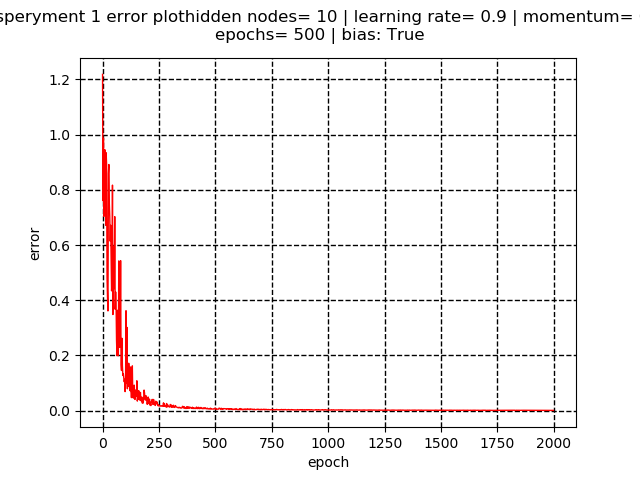
\includegraphics{imgs/11.png}\\
Podpunkt 1.2\\
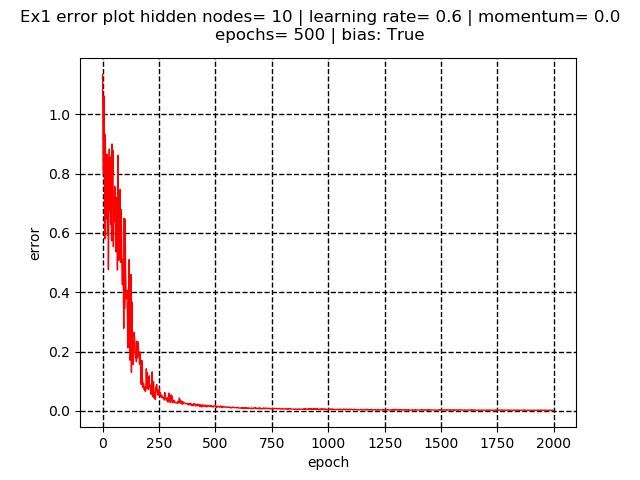
\includegraphics{imgs/12.png}\\
Podpunkt 1.3\\
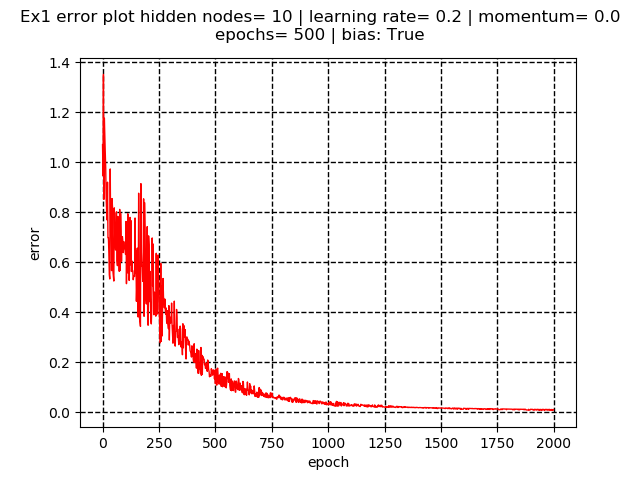
\includegraphics{imgs/13.png}\\
Podpunkt 1.4\\
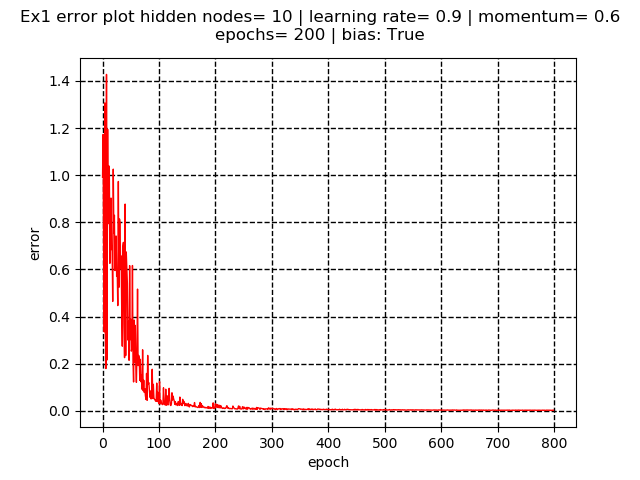
\includegraphics{imgs/14.png}\\
Podpunkt 1.5\\
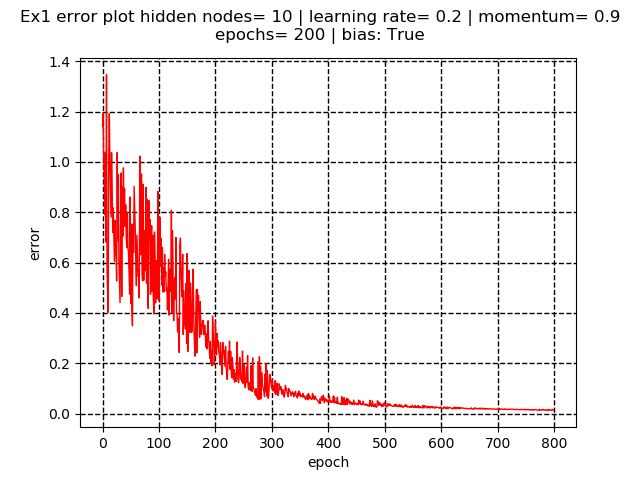
\includegraphics{imgs/15.png}\\
}  

{Eksperyment 2\\
Podpunkt 2.1\\
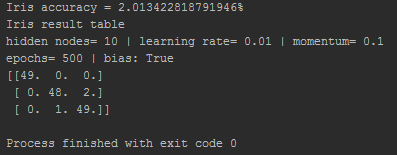
\includegraphics{imgs/211.png}\\
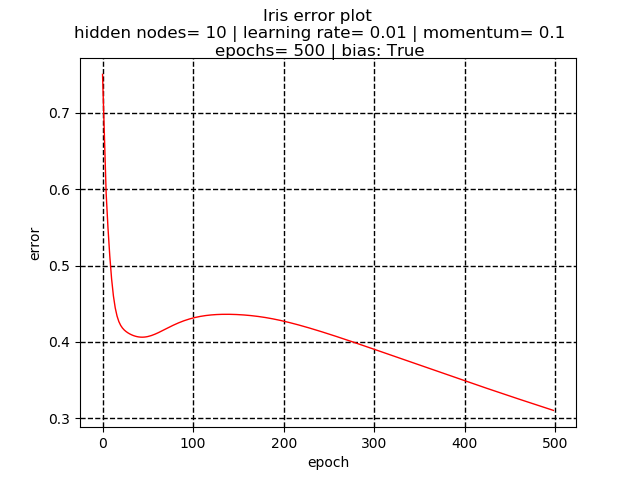
\includegraphics{imgs/212.png}\\
Podpunkt 2.2\\
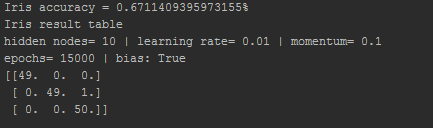
\includegraphics{imgs/221.png}\\
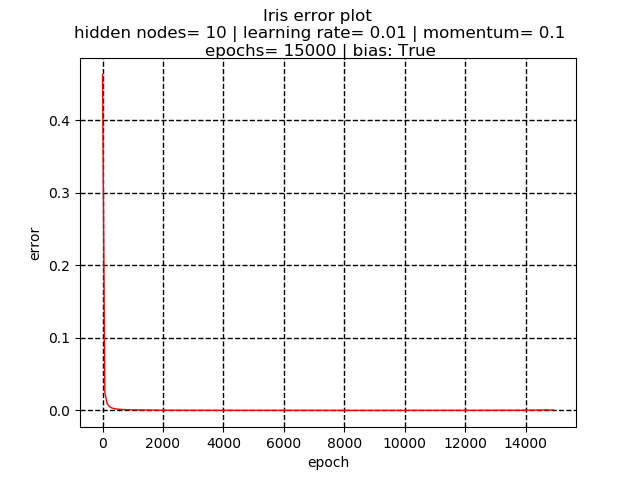
\includegraphics{imgs/222.png}\\
Podpunkt 2.3\\
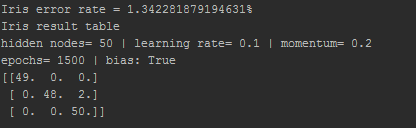
\includegraphics{imgs/231.png}\\
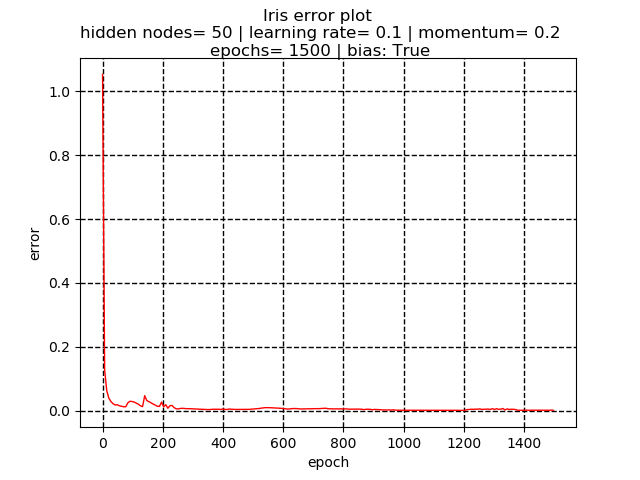
\includegraphics{imgs/232.png}\\
Podpunkt 2.4\\
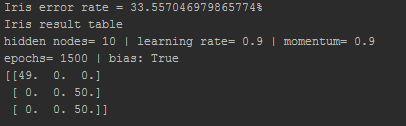
\includegraphics{imgs/241.png}\\
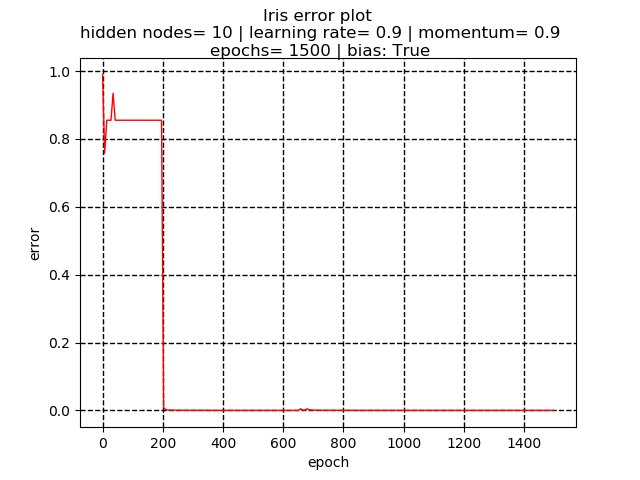
\includegraphics{imgs/242.png}\\
Podpunkt 2.5\\
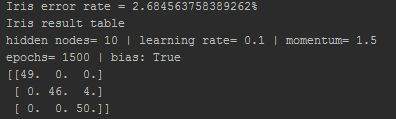
\includegraphics{imgs/251.png}\\
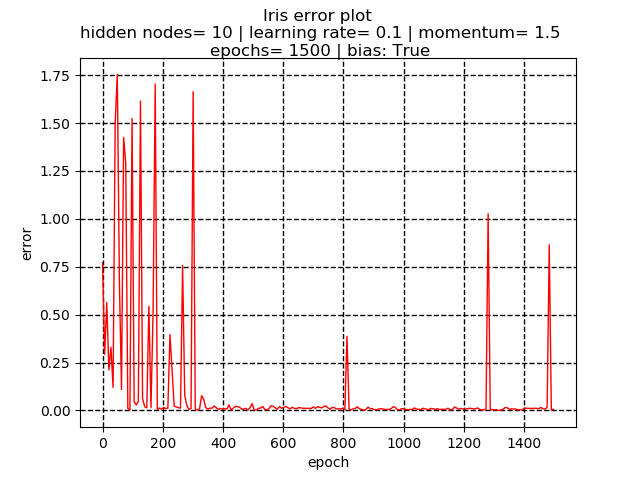
\includegraphics{imgs/252.png}\\
Podpunkt 2.6\\
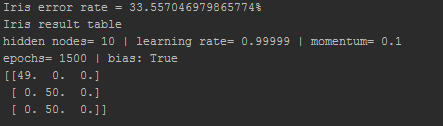
\includegraphics{imgs/261.png}\\
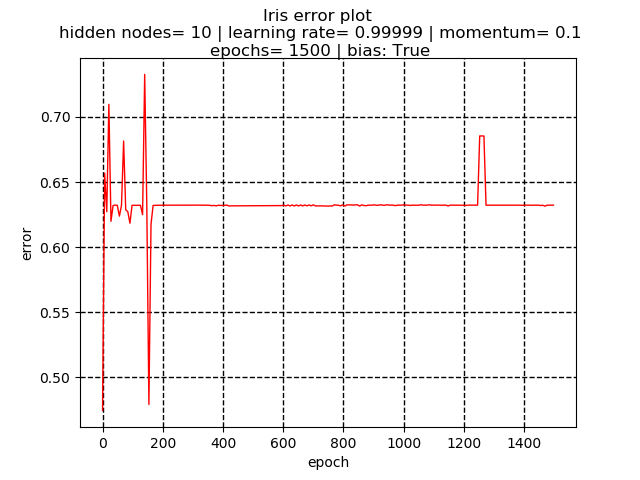
\includegraphics{imgs/262.png}\\
}

{Eksperyment 3\\
Podpunkt 3.1\\
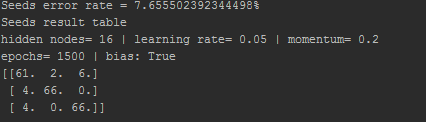
\includegraphics{imgs/311.png}\\
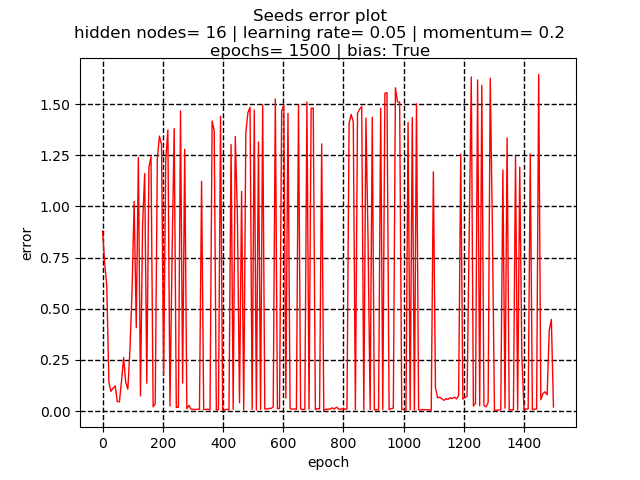
\includegraphics{imgs/312.png}\\
Podpunkt 3.2\\
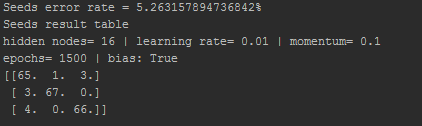
\includegraphics{imgs/321.png}\\
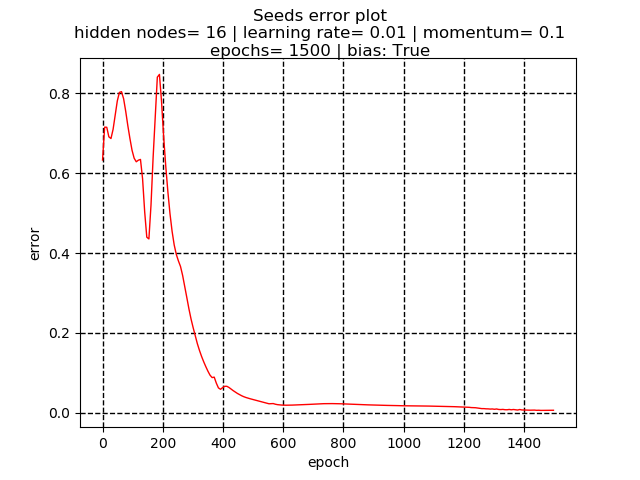
\includegraphics{imgs/322.png}\\
Podpunkt 3.3\\
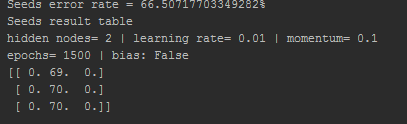
\includegraphics{imgs/331.png}\\
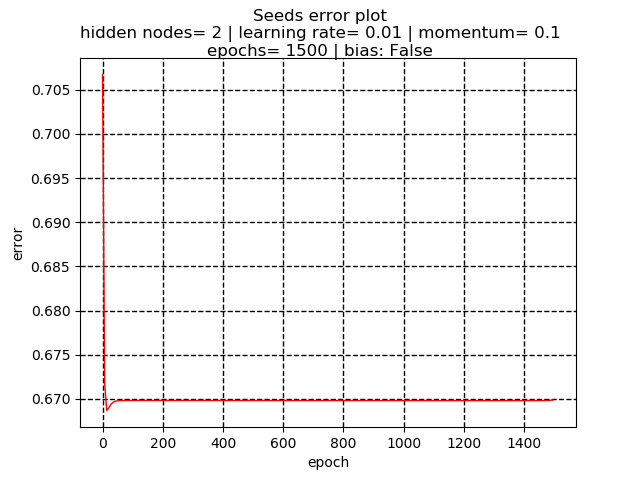
\includegraphics{imgs/332.png}\\
Podpunkt 3.4\\
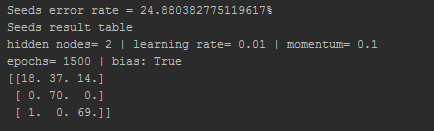
\includegraphics{imgs/341.png}\\
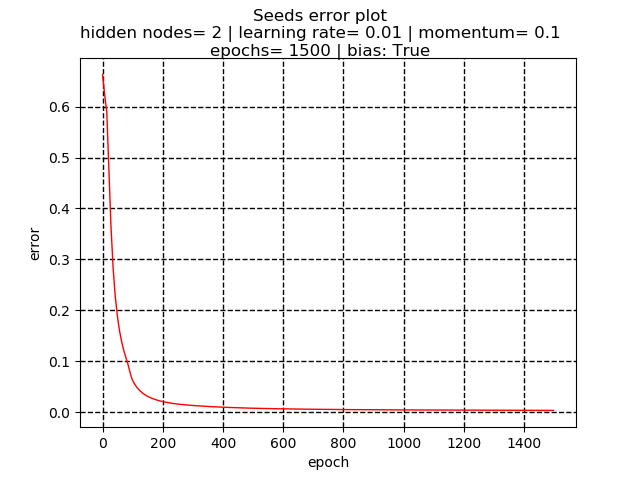
\includegraphics{imgs/342.png}\\
}

{Eksperyment 4\\
Podpunkt 4.1\\
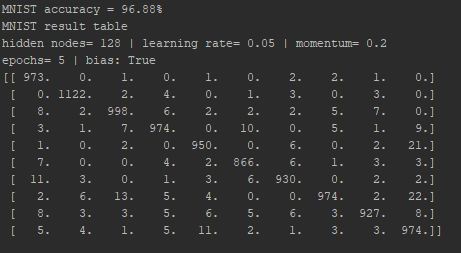
\includegraphics{imgs/MNIST1_1.png}\\
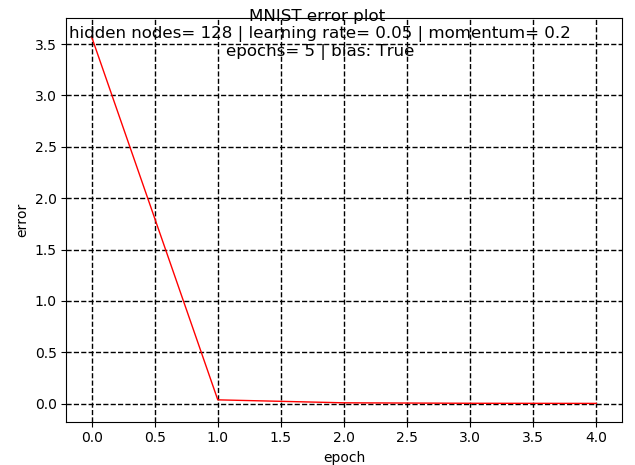
\includegraphics{imgs/MNIST1.png}\\
}

{Eksperyment 5\\
Podpunkt 4.1\\
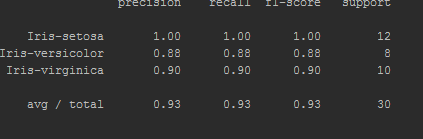
\includegraphics{imgs/KNN11.png}\\
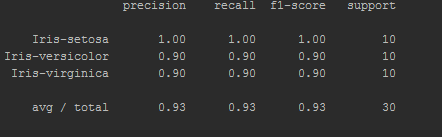
\includegraphics{imgs/KNN21.png}\\
}




\section{Dyskusja}
{\color{blue}
Sekcja ta powinna zawierać dokładną interpretację uzyskanych wyników
eksperymentów wraz ze szczegółowymi wnioskami z nich płynącymi. Najcenniejsze
są, rzecz jasna, wnioski o charakterze uniwersalnym, które mogą być istotne
przy innych, podobnych zadaniach. Należy również omówić i wyjaśnić wszystkie
napotkane problemy (jeśli takie były). Każdy wniosek powinien mieć poparcie we
wcześniej przeprowadzonych eksperymentach (odwołania do konkretnych wyników).
Jest to jedna z najważniejszych sekcji tego sprawozdania, gdyż prezentuje
poziom zrozumienia badanego problemu.}

\section{Wnioski}
{\color{blue}
W tej, przedostatniej, sekcji należy zamieścić podsumowanie najważniejszych
wniosków z sekcji poprzedniej. Najlepiej jest je po prostu wypunktować. Znów,
tak jak poprzednio, najistotniejsze są wnioski o charakterze uniwersalnym.}

\begin{thebibliography}{0}
  \bibitem{l2short} T. Oetiker, H. Partl, I. Hyna, E. Schlegl.
    \textsl{Nie za krótkie wprowadzenie do systemu \LaTeX2e}, 2007, dostępny
    online.

\bibitem{wiki} 
\texttt{https://pl.wikipedia.org/wiki/Perceptron\_wielowarstwowy}

\bibitem{irisi} 
\texttt{http://archive.ics.uci.edu/ml/datasets/Iris}



\end{thebibliography}


\end{document}
